%                                   PREAMBLE

\documentclass[a4paper,10pt,twocolumn]{article}

\usepackage{amsthm}
\newtheorem{prop}{Proposition}
\theoremstyle{definition}
\newtheorem{defn}{Definition}

\usepackage{minted}

\usepackage{enumitem}
\usepackage{graphicx}

\usepackage{tikz}
\usetikzlibrary{arrows.meta, positioning, fit, patterns, shapes.geometric,
  shapes.multipart}

% Typographical tweaks
\usepackage{microtype}

% XXX Cursed settings
\usepackage[style=authoryear-icomp,maxcitenames=1,maxbibnames=999,uniquename=false,uniquelist=false]{biblatex}
%\usepackage{biblatex}
\addbibresource{report.bib}

\ifdefined\isdraftmode
  \usepackage{todonotes}
\else
  \usepackage[disable]{todonotes}
\fi

% Style taken from the ACM Primary Article template.
\usepackage{unicode-math}
\setmathfont[Scale=MatchUppercase]{LibertinusMath-Regular.otf}
\usepackage[tt=false]{libertine}
\setmonofont[StylisticSet=3]{inconsolata}

% Should be at the end, for some reason
\ifdefined\isdraftmode
  \usepackage[hidelinks]{hyperref}
\else
  \usepackage{hyperref}
\fi
\usepackage{cleveref}

\frenchspacing
\newcommand*{\code}{\texttt}
\newcommand*{\acronym}{\textsc}
\newcommand*{\IsabelleHOL}{Isabelle/\acronym{Hol}}
\newcommand*{\API}{\acronym{Api}}
\newcommand*{\WASM}{\acronym{Wasm}}

\newcommand*{\hoare}[3]{%
  \left\{\,{#1}\,\right\}
  \mathrel{#2}\nolinebreak
  \left\{\,{#3}\,\right\}
}
\DeclareMathOperator{\usage}{usage}
\DeclareMathOperator{\execscf}{exec\_scf}

%                                   DOCUMENT

\title{
  Exploiting Microarchitectural Timing Channels from JavaScript \\
  \acronym{Comp}6841 Project Report}
\author{Thomas Liang \\ z5418574 \\ \textsf{thomas.liang@unsw.edu.au}} % XXX

\begin{document}
\maketitle

\section{Results}

My project was to attempt to replicate a timing channel attack described by
\textcite{Oren_KSK_2015}, and to research and test possible improvements on
their attack method.
I will refer to this project as ``the paper'' or ``the attack''.

% Because the source code for the attack is not public, there was no existing
% reference code to draw from.
% I needed to build a deep understanding of the attack from the paper and other
% readings, and then continually experiment, measure, and iterate on my method.

I completed my project with some success:
\begin{itemize}[nosep]
\item I demonstrated the presence of cache-based timing channels measurable
  inside JavaScript
\item I used Python and Matplotlib to analyse the exact effect of those timing
  channels
\item I applied my knowledge of systems programming, and data structures to
  optimise the performance of my implementation of the cache-profiling algorithm
\end{itemize}
For what it's worth, I also contacted the first author of the paper I am
referencing, Dr Yossef Oren, about my project asking for advice.
Part of our correspondence is presented in Appendix B.

However, other parts of my project had limited results:
\begin{itemize}[nosep]
\item My attempt to improve on their method by using WebAssembly failed, due to
  a mistake when checking browser compatibility.
\item My cache-profiling algorithm seems to work, but I could not optimise it
  enough to run in a feasible time for an attack.
\end{itemize}
I reflect on what I would have done differently in \Cref{sec:challenged}.

% Overall, this project taught me skills across a range of disciplines.
% In particular, I want to emphasise that I learnt about:
% \begin{itemize}[nosep]
%   \item \acronym{Cpu} architecture, particularly how set-associative caches
% work, which are used in all modern x86 Intel and \acronym{Amd} processors
%   \item Optimising JavaScript code, by learning about the behaviour of
%     \acronym{jit} compilers, and the internals of the Firefox JavaScript engine
%     SpiderMonkey, and
%   \item The history of browser security, the wide range of security mechanisms
%     modern browsers contain, and why creating a sandbox is so difficult.
% \end{itemize}

% In this report, I will briefly outline the technical basis for the attack and
% its components, my experience replicating the attack, and ...
% In the appendix, I include:
% \begin{itemize}[nosep]
% \item A link to the artifacts for my project
% \item Some of the emails I exchanged with Dr Oren
% \item a rough timeline of my project, and
% \item The Matplotlib visualisations of the above-mentioned analysis
% \end{itemize}

\section{What I did}

In this section, I outline the technical foundations for the attack I am
replicating, and what algorithms I implemented.

\subsection{Background for the Attack}

To speed-up reads from memory, \acronym{cpu}s contain \emph{caches}, which store
the values of memory addresses accessed recently.
Caches lower the cost of reading from memory from hundreds to single-digit
nanoseconds.
If a value is present in the cache, that is called a \emph{cache hit}, and if
not, it is a \emph{cache miss}.

Usually, all the processes on a machine will have their own allocation of memory
from the operating system, but share the same cache.
This means a process' performance can be impacted by other processes evicting
its values from cache.

% Your web browser executes JavaScript (JS) code in an isolated environment that should
% not be able to communicate outside its process, yet security researchers have
% exploited Web \API{}s to leak information to and also to spy on the rest of your
% machine.
% On paper, it should be safe to execute arbitrary JS code downloaded from
% the websites you visit (and the vast majority of web users do so!).
% However, the interface exposed by your browser (so-called Web \API{}s) are full
% of \emph{side-channels}, from the time it takes to load videos, and for this
% project, the time it takes to access a variable, which malicious code can
% exploit to learn information.

In 2015, \textcite{Oren_KSK_2015} showed that by measuring the impact of cache
misses, JS code could accurately predict \emph{what other websites the
  browser had open on other tabs.}
% , and (2) hardware events, such as mouse activity,
% and even the motion of a user in front of a laptop.
By using the High Resolution Time API, which gave timestamps with
nanosecond-resolution, JS code could detect cache misses.
% determine what elements of a buffer were part
% of the same \emph{cache set}.
By monitoring accesses to certain cache sets, the authors could determine a
unique memory-access ``fingerprint'' for different popular websites.
% and that
% are triggered by hardware events.
According to my private correspondence with Dr Oren, as a result of this paper
and other work, browser vendors quickly lowered the resolution of time that
JavaScript code had access to.

The attack I was replicating was a turning point in web security, as it showed
that JavaScript code executed in a browser context was able to detect the
behaviour of the rest of the browser and computer.
Merely by loading the website, a user was at risk.
% It did so by measuring and exploiting timing variations caused by the
% \acronym{cpu} cache present in early Intel Core \acronym{cpu}s.

I refer the interested reader to the paper itself, for the details of the
algorithm.

\subsection{Implementation Details}

% My primary focus was on implementing Algorithm 1 from the paper.
% which is the
% heuristic algorithm that finds an ``eviction set'' for a particular victim variable.
% The eviction set is a set of offsets into the eviction buffer (16 offsets, for
% the i7-6600U) that are in the same cache set as the victim.
% Thus, by accessing each of those offsets, we can guarantee that the cache set is
% \emph{primed}, and only contains values from addresses in the attacker's memory
% allocation.

First, I sought out to measure the timing variation caused by cache misses
overall.
I adapted a method from Ana Dumitras' dissertation, which cited
\textcite{Oren_KSK_2015} and had some short test code.
% This is essential information for calibrating the cache-profiling algorithm.
% Fortunately, I found \code{an4/Spy}\footnote{\url{https://github.com/an4/Spy}},
% a GitHub repository containing the artifacts for Ana Dumitras' dissertation on a
% web timing attack.
% She cites \textcite{Oren_KSK_2015}, and provides some code to measure the timing
% variations.
% I adapted that code into my own style, rewriting it in TypeScript.

The algorithms outlined in the paper are \emph{heuristics}.%, and so do not
always succeed.
The JavaScript runtime will touch the cache in unpredictable ways,
interfering with our measurements.
It is important that we minimise every unnecessary function call or memory
access, since that might hurt the accuracy of our algorithm.

I sought out to implement Algorithm 1.
Algorithm 1 is a computationally-intensive algorithm, and so required many
optimisations:
% Next, I sought out to implement Algorithm 1.
% The primary difficulty for this part was all the optimisations required.
% I made a major error in that I skipped over Optimisation \#1 listed in the paper,
% which reduces the search space for the algorithm from over 131K offsets to just 8K.
% Embarrassingly, I only discovered this in the final week of the project.
% Other optimisations I learnt about are as follows:


\paragraph{Just-In-Time compilation.}
Because the JS engine in Firefox is a
Just-In-Time (\acronym{jit}) compiler, code is progressively optimised as it is
run.
We need to ``warm-up'' the code for accurate measurements.

% When code is run, the engine learns to perform more optimisations based on
% what types each variable can hold, what fields objects have, etc.
% This means that it is essential to run your benchmarking code at least a few
% times to ``warm-up'' the code, to let the engine optimise it, for an
% accurate measurement.

\paragraph{\code{var} versus \code{let} bindings.}
% There are two ways of declaring mutable variable bindings in JS, with the
% older \code{var} or newer \code{let} form.
A variable declared with \code{var} has scope of the surrounding function body,
whereas a \code{let} binding has scope the enclosing block.
If you declared a variable with \code{let} in the initialisation expression of a
\code{for} loop, unoptimised engines would then \emph{re-declare your variable
on every iteration}.
My code was faster when using \code{var}, with all variables declared outside
the hot loop.

% An unfortunate consequence of this caused performance disparities in early
% JavaScript engines including NodeJS, between \code{for} loops that used
% \code{var} versus \code{let}.
% If you used \code{let} to declare a variable in a \code{for}-loop, its scope was
% just the loop body.
% Firefox 34 is so old that changing all my uses of \code{let} to \code{var}
% caused a noticeable change in performance.
% To be safe, all variables in hot loops are ``pre-allocated'', by being declared
% but uninitialised prior to the loop.
% This would be considered bad practise in modern software engineering, but
% essential for this attack.
% 
% I learnt about SpiderMonkey internals from the official
% documentation\footnote{\url{https://spidermonkey.dev/docs/}}.

\paragraph{Avoiding compiler optimisations}
Another minor issue is that in order to manipulate the cache into the state we
want, we must perform many meaningless memory accesses.
% However, we do not really do anything with the values returned by those
% accesses.
To a clever compiler, these accesses an be replaced in a process called
\emph{constant-folding}.
Thus, it's necessary to obfuscate your code, such as using
\code{std::hint::black\_box} in Rust.
% in ways that the compiler does not
% realise the accesses are pointless.

% In Rust, this occurred as calls to \code{std::hint::black\_box}, a function for
% writing benchmarks.%that tells the compiler to be ``maximally pessimistic'' about
% what the function could possible do.
% In JS, rather than just reading from memory, we treat the eviction buffer like a
% linked list, where each element ``pointed'' to the next element.
% Each value in the array ``pointed'' to the next element, and so we iterated
% through the buffer as if we were traversing a linked list.

\paragraph{Linked lists}
As mentioned above, in order to minimise the amount of touched memory during the
cache profiling process, I implemented my own linked list.
% This meant insertions and deletions only required one memory access.
% Na\"ively, we might implement the cache set using a JS Array, which is backed by
% a contiguous memory buffer.
% However, to insert elements to the front, that would cause all the elements to
% have to be shifted, touching a lot of memory addresses.
% Instead, I used a linked list, so that when we are removing an offset from the
% cache set, we only had to touch one field of the list.

\paragraph{\WASM{} optimisation.}
I tried to lower the cache interference by the JS runtime by writing the code in
WebAssembly (\WASM{})\footnote{\url{https://webassembly.org/}}.
% However, this idea ultimately failed.

% , a relatively-new
% format for web programming language that is similar to native machine code.
% The hope is that by using \WASM{} we can have maximum control over what the browser
% does while executing the attack, and minimise cache interference.

% To generate \WASM{} code, I chose to use Rust, a programming language that is
% gaining popularity for low-level systems programming.
% Rust was the natural choice for a few reasons:
% it provides a type system that is explicit about casting between
% integer sizes, which is essential for the tricky memory accesses our algorithms
% do;
% Rust is likely the language with the most comprehensive \WASM{} story after C/C++.
% This required spending time learning how to set up a Rust and \WASM{} toolchain,
% using libraries like \code{wasm-bindgen}.
% 

\subsection{Findings}
Here is a collection of things I learnt while trying to implement the project.

\paragraph{Browser versioning is hard}

In order to use \WASM{}, I tested my code on Firefox 52.
According to Can I use...,\footnote{\url{https://caniuse.com/}} Firefox 15-54
supported the High Resolution Time API \parencite{caniuse}.
However, only later I discovered that Firefox 52 is a new enough version that the timer
resolution had already been silently lowered to mitigate timing-based attacks.
\footnote{I could not identify the exact version where this happened, but this
is verifiable by running Firefox 52 and checking the output of
\code{Performance.now}.}
% My attempt to implement the algorithm using Rust and \WASM{} failed because of
% browser incompatibilities that I was unaware of.
% I sourced my information about what technologies and \API{}s a browser
% version supported from Can I use....
%a free
%online database about browser support.

% The vulnerability identified by the paper depends on the High Resolution Time
% \API{}.
%which manifests as the function \code{Performance.now()}.
% On Firefox 34, the version the authors demonstrated the attack on,
% \code{Performance.now()} returned a timestamp with nanosecond-resolution.
% This level of precision is essential to the attack.
% 
% The first version of Firefox to support \WASM{} is Firefox 52.
%It seems that Firefox 52 would be the perfect attack target.


\paragraph{Secretly priming the cache is hard}

% The final obstacle that made my project unfeasible as an attack is because of
% the necessity to \emph{prime} the cache.
% An attacker primes the cache by accessing enough memory addresses to overwrite all parts
% of the cache with its own memory.
% That way, if another process changes the cache, the attacker will get cache misses.

Priming the cache requires so much \acronym{cpu} work it can freeze the
whole browser.
% Because old browsers are often single-threaded, which is supported by the
% cooperative multithreading environment provided by JS, doing a lot of work on
% the \acronym{cpu} can freeze the whole browser.
You can mitigate this by manually adding yield points to a hot loop with
\code{setTimeout}.
However, the minimum timeout is 4 ms, which is very expensive when we are
measuring phenomenon in nanoseconds.
% On Firefox 34, the only way to do so is to use \code{setTimeout}, which will run
% the provided callback function after a set number of milliseconds.
% However, according to the HTML standard, the minimum passed timeout is 4 ms.
% That means adding a yield point to a loop will incur a 4 ms penalty each time.
% When we are measuring timing variations to the nearest nanosecond, one millionth
% of a millisecond, that cost is an eternity.

% When a script is taking up all the \code{cpu} of the process, browsers are
% clever enough to ask the user if they would like to end the process.
% That would stop my implementation of the attack in its tracks.

\section{How I was Challenged}
\label{sec:challenged}

I chose this project because it is tangentially related to my Honours thesis: I
am working at TS\footnote{\url{https://trustworthy.systems/}}, as part of the
work to show that seL4\footnote{\url{https://sel4.systems/}} is free of timing channels.

As someone interested in pursuing research as a career, I wanted to push myself
to do more research.
This project asked me to use my academic skills to read dense technical
literature, and apply my background knowledge from my OS courses and Honours
thesis.
I think in hindsight, I should have read through a wider range of literature, to
find a procedure that was more feasible within the timeframe.
% I found the paper by \textcite{Oren_KSK_2015} from a survey paper I knew about
% from my Honours project, \textcite{Ge_YCH_18}.
It was difficult to replicate this attack due to the lack of reference code, and
because it is a conference paper, so it lacks detail compared to a full journal article.

The primary challenge I faced was that I was constantly slowed by technological incompatibilities:
\begin{itemize}
  \item The Rust compiler and LLVM emit \WASM{} code that uses extensions
    unavailable in the versions of Firefox I targeted.
  \item Mozilla silently decreased the precision of the High Resolution Time
    \API{} sometime after Firefox 34.
  \item I could not find a compatible version of VMWare Fusion. I could not get
    Ubuntu 14.04 running on UTM, and resorted to the much slower hypervisor
    VirtualBox, which impacted my measurements.
%   \item Writing JS in a pre-ES2015 style is awful.
%     You do not have access to \code{Promise} objects, let alone
%     \code{async}/\code{await} syntax.
%   \item I needed to acquire an Intel Core machine to test this project, but I
%     developed on a different machine, which slowed my development workflow.
\end{itemize}
In hindsight, I think I underestimated the cost that all the prerequisites of
this project would bring.
Acquiring an Intel test machine, setting up virtual machines, and the
infrastructure for three programming languages(Rust, \WASM{}, TypeScript) cost
several weeks, which are crucial in the short timeframe of this project.

I tried to implement my Rust/\WASM{} algorithm \emph{before} I had demonstrated
the result just using JavaScript.
As a result,
\begin{itemize}
\item I lost time because the \WASM{} direction was futile.
\item I tried to implement an algorithm I didn't yet fully understand until I
  tried to do so in JS.
  % I completely missed the existence of Optimisation 1, for example.
\end{itemize}
I definitely should have applied what I learnt about always getting the Minimum
Viable Product first, and not gotten over-excited about the project.

% Given the chance to do this project again, I would have chosen a project that I
% could have more easily developed on my own machine on a less niche target.
% I would have curbed my overconfidence.

\appendix
\section{Project Timeline}

\begin{description}
\item[Week 3]
  I spent the week trying to acquire a machine to test my attack on.
  The authors demonstrated the attack on 2nd-5th generation Intel Core
  CPUs, and the algorithm they described relies on behaviour unique to the
  caches on Intel Core.
  I needed to find a machine with a CPU of a similarly old generation, such that
  its cache organisation had been reverse-engineered and made public online.
  Luckily, my partner had an old MacBook Pro with an Intel Core i7-6600U, which
  matched those requirements.
\item[Week 4]
  Trying to set up a VM.
  The paper demonstrates the attack on Ubuntu 14.04 running on VMWare Fusion 7.
  That version of Fusion is no longer officially available.
  The MacBook Pro I was testing my code on ran MacOS Big Sur, which was too old
  for the oldest available version of Fusion.
  The only other two hypervisor options were UTM or VirtualBox.
  I had various graphics incompatibilities with UTM and Ubuntu 14.04, so I had
  to use VirtualBox.
\item[Week 5]
  Implementing the Rust version.
  I followed a Rust and WebAssembly tutorial, and read a lot about WebAssembly
  internals.
  I lost a lot of time because the newest version of the Rust compiler and LLVM
  use \WASM{} extensions that are not supported by Firefox 52.
  I learnt about \WASM{} validation techniques, and about the various
  extensions.
  See \code{tc-spy-wasm/Makefile} for how we eliminate use of the Reference
  Types and Sign-Extension Operators \WASM{} extensions.

  Ultimately it was in vain, because the High Resolution Time \API{} had its
  resolution reduced by Firefox 52, so the attack was no longer possible.
\item[Week 6]
  Reimplementing the JS version, using just what the paper describes.
  Side quests included implementing my own linked list in JS to make removing
  from the cache set as fast as possible.
\item [Week 7]
  Hopelessly trying to optimise the above implementation.
  Rewriting to have the various optimisations described above.
\item [Week 8]
  Writing this report.
\end{description}

\newpage
\onecolumn
\section{Correspondence with Dr Oren}

\begin{center}
  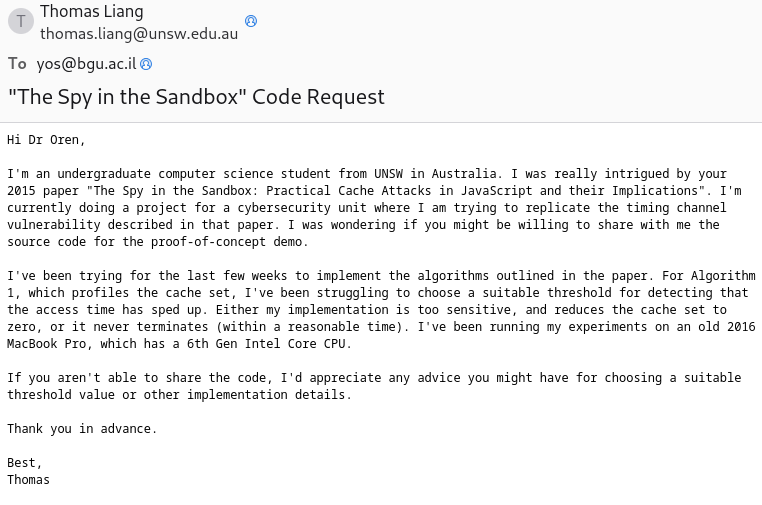
\includegraphics[width=0.5\textwidth]{email-to-oren.png}
\end{center}

\begin{center}
  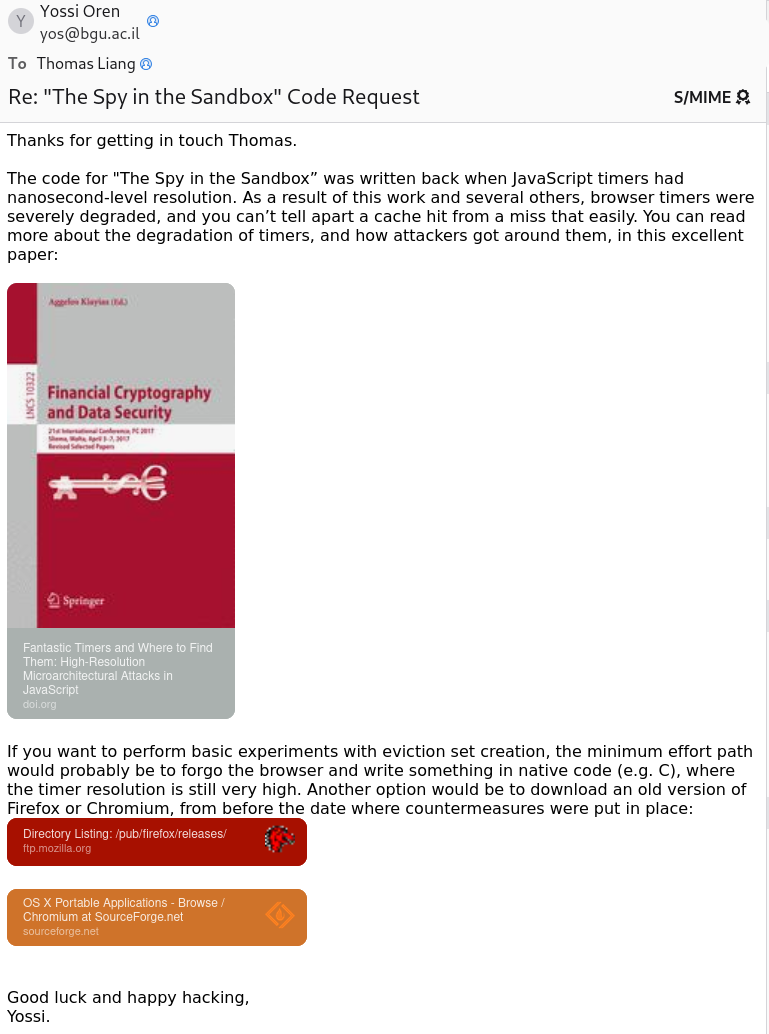
\includegraphics[width=0.5\textwidth]{reply-from-oren.png}
\end{center}

\section{Link to artifact}

You can find all the artifacts for this project at the following GitHub
repository: \url{https://github.com/ShunyaoLiang/comp6841-sap}.

My Rust implementation can be seen in the \code{tc-spy-wasm} folder of the
artifacts respository.

\section{Matplotlib Visualisations}

\begin{figure}[h]
  \centering
  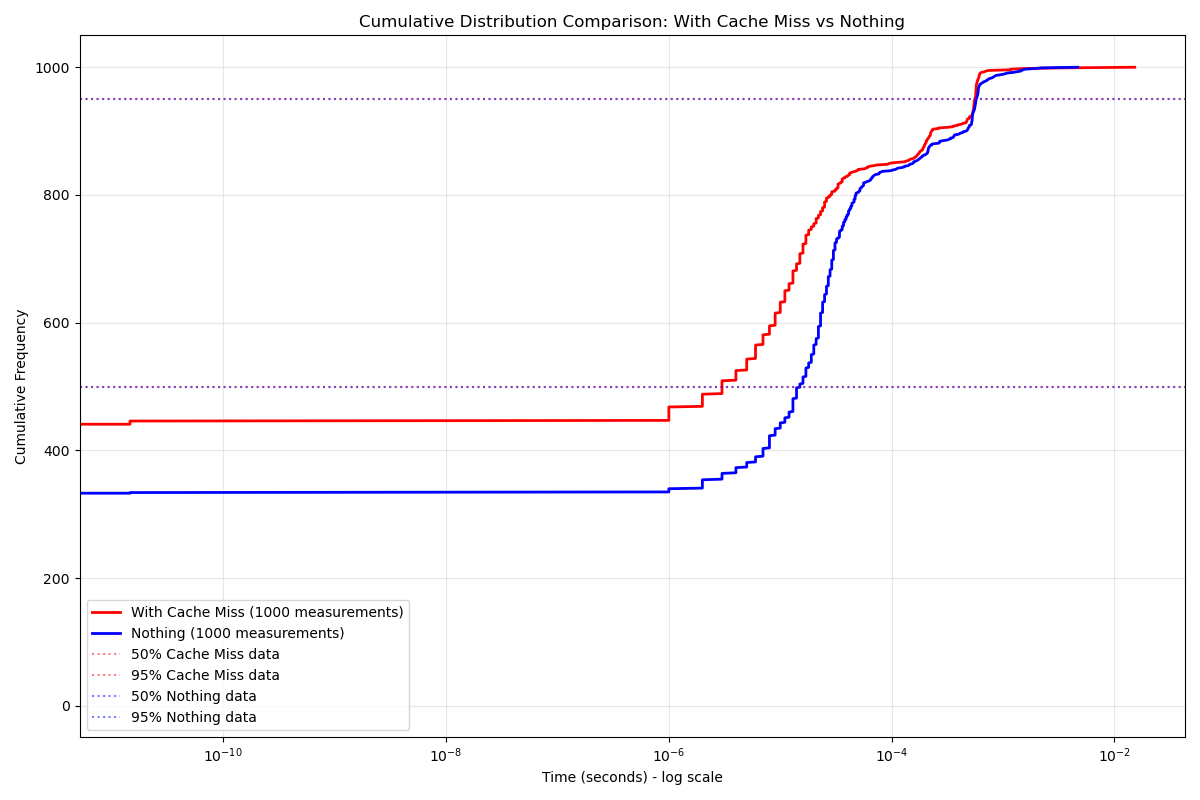
\includegraphics[width=0.8\textwidth]{../2025-07-20-comparison-nonsense.png}
  \caption{Data from measuring the impact of cache misses.}
\end{figure}

Here is a figure from when I was calibrating the cache profiling algorithm.
It plots the cumulative frequency graph of the time difference caused by a cache
miss versus a cache hit (called ``nothing'').
Clearly, there is some statistical significance and the cache hit causes some impact.


\section{Code excerpts I am proud of}

Below are snippets of code that demonstrate some of the deep technical work I did.

\begin{figure}[h]
  \begin{minted}{TypeScript}

function findEvictionSet(fuel: number, threshold: number): object {
    threshold /= NS_PER_MS;
    console.log('Starting cache profiling...');

    initEvictionBuffer(primeView);
    var cacheSet = newCacheSet();
    // Find a better name for [results].
    var results = profileCacheSet(cacheSet, 500, threshold).evictionSet as { address: number, speedUp: number }[];
    console.log(results);
    var bestResult = results.reduce((a, b) => a.speedUp > b.speedUp ? a : b);
    // The address that had the highest speed up is probably a squatter address.
    var squatterAddress = bestResult.address;
    var squatterSpeedUp = bestResult.speedUp;
    if (squatterAddress === undefined) {
        throw new Error("Failed to find squatter address");
    }
    console.log(`Found squatter address [0x${squatterAddress.toString(16)}] with speed up [${squatterSpeedUp}].`);
    // All possible other offsets that are in the same cache set as the victim
    // and the squatter address must have the same bits at positions 6-12.
    // [0xfc0] is [0b1111_1100_0000].
    cacheSet = newCacheSet().filter(addr => (addr & 0xfc0) === (squatterAddress & 0xfc0));
    for (var i = 0; i < cacheSet.length - 1; ++i) {
        primeView.setUint32(cacheSet[i] as number, cacheSet[i + 1] as number);
    }
    primeView.setUint32(cacheSet[cacheSet.length - 1] as number, cacheSet[0] as number);
    shuffleArray(cacheSet);
    console.log(`Reduced cache set has length [${cacheSet.length}]. (Should be 8192.)`);

    return profileCacheSet(cacheSet, fuel, threshold);
}
\end{minted}
  \caption{The cache-profiling algorithm, in TypeScript.}
\end{figure} 

\begin{figure}[h]
\begin{minted}{Makefile}
# From rust-lang/rust issue #128475.
# https://github.com/rust-lang/rust/issues/128475
RUSTFLAGS+=-C target-cpu=mvp
CARGOFLAGS+=-Z build-std=std,panic_abort

# From rust-lang/rust issue #109807
# https://github.com/rust-lang/rust/issues/109807
RUSTFLAGS+=-C target-feature=-sign-ext

.PHONY: build
build:
	RUSTFLAGS="$(RUSTFLAGS)" wasm-pack build --debug --target no-modules \
		. $(CARGOFLAGS)
	wasm-validate \
		--disable-reference-types \
		--disable-sign-extension \
		pkg/tc_spy_wasm_bg.wasm
	wasm2wat pkg/tc_spy_wasm_bg.wasm > pkg/tc_spy_wasm_bg.wat
\end{minted}
  \begin{minted}{toml}

# Ensures that we do not use the sign-extensions operators WASM extension.
# https://github.com/rust-lang/rust/issues/109807#issuecomment-1704431724
[package.metadata.wasm-pack.profile.dev]
wasm-opt = ["--signext-lowering"]
[package.metadata.wasm-pack.profile.profiling]
wasm-opt = ["--signext-lowering"]
[package.metadata.wasm-pack.profile.release]
wasm-opt = ["--signext-lowering"]
\end{minted}
  \caption{The amount of work it takes to generate \WASM{} code compatible with
    old versions of Firefox.}
\end{figure}

\begin{figure}[h]
\begin{minted}{Rust}
fn access_victim_variable(victim: &Box<u32>) -> u32 {
    let ptr = black_box(victim.as_ref() as *const u32);
    // Safety: This function is only called to read from boxed variables we own.
    let value = unsafe { black_box(std::ptr::read_volatile(ptr)) };
    black_box(value)
}
\end{minted}

  \begin{minted}{Rust}
            let t1 = {
                let before = self.performance.now();
                black_box(access_victim_variable(&self.victim));
                self.performance.now() - before
            };
\end{minted}
  \caption{How to read a variable s.t. it definitely is not optimised out in Rust.}
\end{figure}


\begin{figure}[h]
\begin{minted}{TypeScript}
interface List {
    head: ListNode | null,
    tail: ListNode | null,
    length: number,
}

interface ListNode {
    value: number,
    next: ListNode | null,
}

function appendToList(list: List, value: number) {
    var node = newNode(value);
    ++list.length;
    if (list.head === null) {
        list.head = node;
        list.tail = node;
    } else if (list.head === list.tail) {
        list.head.next = node;
        list.tail = node;
    } else {
        if (list.tail !== null) {
            list.tail.next = node;
            list.tail = node;
        } else {
            unreachable();
        }
    }
}

function popFromList(list: List): number {
    if (list.head !== null) {
        var ret = list.head.value;
        list.head = list.head.next;
        --list.length;
        return ret;
    }
    unreachable();
}
\end{minted}
  \caption{Linked lists in TypeScript, before \code{class} syntax exists.}
\end{figure}

\twocolumn
\printbibliography



\end{document}
